\documentclass{article}
% \usepackage[english]{babel}

\usepackage{polyglossia}
\setdefaultlanguage{english}

\usepackage{fontspec}
\setmainfont[Mapping=tex-text]{LinLibertineO}
\newfontfamily\ipa{LinLibertineO}
\setsansfont[Scale=MatchLowercase]{Carlito}
\setmonofont[Scale=MatchLowercase]{DejaVu Sans Mono}

\usepackage[a4paper,bottom=3cm,top=2.5cm,foot=1.5cm,left=1.75cm,right=1.75cm]{geometry}

\usepackage{fontspec}
\setmainfont[Mapping=tex-text]{LinLibertineO}
\newfontfamily\ipa{LinLibertineO}
\setsansfont[Scale=MatchLowercase]{Carlito}
\setmonofont[Scale=MatchLowercase]{DejaVu Sans Mono}

\usepackage{url}
\usepackage{graphicx}
\usepackage{longtable}

\usepackage{color}
\usepackage{colortbl}

\usepackage[table]{xcolor}
\usepackage{booktabs}

\usepackage{lastpage}
\usepackage{datetime}
\usepackage{textpos}
\usepackage{xltxtra}

\definecolor{gris}{rgb}{0.4,0.4,0.4}
\definecolor{morado}{cmyk}{0.09,1,0,0.3}
\definecolor{azul}{cmyk}{1,0.64,0,0.06}


\usepackage{fancyhdr}
\pagestyle{fancy}

% headers y footers
% borramos los estandares
\fancyhf{}
% y le sacamos esa horrible raya que viene por default
\renewcommand{\headrulewidth}{0pt}
\renewcommand{\footrulewidth}{0pt}

% numero de pagina
\fancyfoot[R]{\oldstylenums{\thepage}/\oldstylenums{\pageref{LastPage}}\quad\quad}

\usepackage{hyperref}
\hypersetup{pdftitle={Ramiro Vignolo--Curriculum Vitae}, pdfauthor={Ramiro Vignolo}, pdfkeywords={}, pdfborder={0 0 0}}

% background
\usepackage{eso-pic}
\newcommand\BackgroundPic{
\put(0,0){
\parbox[b][\paperheight]{\paperwidth}{%
\vfill
\centering

\includegraphics{logos/back.pdf}%
\vfill
}}}

% longitudes
\newlength{\chico}
\setlength{\chico}{0.5cm}

\newlength{\grande}
\setlength{\grande}{1.0cm}

\newlength{\ancholeft}
\setlength{\ancholeft}{1.7cm}
\newlength{\anchomain}
\setlength{\anchomain}{13.0cm}
\newlength{\anchoright}
\setlength{\anchoright}{1.5cm}

\newlength{\anchomainright}
\setlength{\anchomainright}{\anchomain}
\addtolength{\anchomainright}{\anchoright}

\newlength{\anchoparrafo}
\setlength{\anchoparrafo}{11.5cm}

\newcommand{\seccionpersonal}[1]{%
\vspace{0.7cm plus 0.2cm minus 0.3cm}
\begin{Large}\textcolor{azul}{\textsc{#1}}\end{Large}
\textcolor{morado}{\hrule}
\vspace{0.2cm plus 0.2cm minus 0.1cm}}

\newcommand{\personalfield}[2]{
\hspace{\chico}\gris{#1}

\smallskip
% \par

\hspace{\grande}{#2}
}



\newenvironment{secciondoscol}[1]{%
% \rowcolors{2}{black!2}{black!0}
\begin{longtable}{p{\ancholeft}p{\anchomainright}}
\multicolumn{2}{l}{
\vspace{0.1cm plus 0.1cm minus 0.1cm}
\hspace{0.25cm}\begin{Large}\textcolor{azul}{\textsc{#1}}\end{Large}
\vspace{-0.1cm}
}
\\
\hline
\vspace{0.2cm plus 0.2cm minus 0.1cm}
\endfirsthead
\multicolumn{2}{l}{
\hspace{0.25cm}\begin{Large}\textcolor{azul}{\textsc{#1}}\end{Large}~~\textcolor{azul}{\textsc{(cont.)}}}\\
\hline 
\vspace{0.2cm plus 0.2cm minus 0.1cm}
\endhead
}{
\end{longtable}
}


\newenvironment{secciontrescol}[1]{%
% \rowcolors{2}{black!2}{black!0}
\begin{longtable}{p{\ancholeft}p{\anchomain}p{\anchoright}}
\multicolumn{3}{l}{
\vspace{0.1cm plus 0.1cm minus 0.1cm}
\hspace{0.25cm}\begin{Large}\textcolor{azul}{\textsc{#1}}\end{Large}
\vspace{-0.1cm}
}
\\
\hline
\vspace{0.2cm plus 0.2cm minus 0.1cm}
\endfirsthead
\multicolumn{3}{l}{
\hspace{0.25cm}\begin{Large}\textcolor{azul}{\textsc{#1}}\end{Large}~~\textcolor{azul}{\textsc{(cont.)}}}\\
\hline 
\vspace{0.2cm plus 0.2cm minus 0.1cm}
\endhead
}{
\end{longtable}
}


\newcommand{\filadosendos}[2]{
 \hfill \textcolor{gris}{\textsf{\small{#1}}} & {\raggedright #2} \\
}
\newcommand{\filadosentres}[2]{
 \hfill \textcolor{gris}{\textsf{\small{#1}}} & \multicolumn{2}{p{\anchomainright}}{\raggedright #2} \\
}
\newcommand{\filatresentres}[4]{
 \hfill \textcolor{gris}{\textsf{\small{#1}}} & {\raggedright #2} & {%
\begin{center}\begin{textblock*}{\linewidth}(0cm,{#4}){#3}\end{textblock*}\end{center}%
} \\
}

\newcommand{\filasep}{ & \\}

% TODO: poner el idioma de babel
\newcommand{\paper}[6]{\filatresentres{#1}{\emph{#3}\\#2\\#4}{\href{#5}{\includegraphics[width=1.2cm]{qr/#6}}}{-0.5cm} \\}
\newcommand{\report}[6]{\filatresentres{#1}{\emph{#3}\\#2\\#4}{\href{#5}{#6}}{-0.5cm} \\}
\newcommand{\congreso}[2]{\filadosentres{#1}{#2}\nopagebreak}
\newcommand{\presentacion}[4]{\filatresentres{}{\emph{#2}\\#1}{\href{#3}{\includegraphics[width=1.2cm]{qr/#4}}}{-0.5cm} \\}
\newcommand{\software}[3]{\filatresentres{#1}{#2}{\href{#3}{\includegraphics[width=1.2cm]{qr/#1}}}{-0.5cm} \\}

\newcommand{\gris}[1]{%
\textcolor{gris}{\textsf{#1}}}

\newcommand{\azul}[1]{%
\textcolor{azul}{\textsf{#1}}}

\newcommand{\titulo}[1]{
\thispagestyle{empty}
\begin{center}
\textcolor{azul}{\Huge{\textbf{#1}}}\\
\vspace{0.1cm plus 0.05cm minus 0.05cm}
\textcolor{gris}{\Large{\textsc{Curriculum Vit\ae}}}
\end{center}
\vspace{0.25cm plus 0.15cm minus 0.1cm}
}

\arrayrulecolor{morado}

% \newcommand{\CC}{C\nolinebreak\hspace{-.05em}\raisebox{.4ex}{\tiny\bf +}\nolinebreak\hspace{-.10em}\raisebox{.4ex}{\tiny\bf +}}
\def\CC{{C\nolinebreak[4]\hspace{-.05em}\raisebox{.4ex}{\tiny\bf ++}}}


\begin{document}
\AddToShipoutPicture{\BackgroundPic}
\titulo{Ramiro Vignolo}

% -=-=-=-=-=-=-=-=-=-=-=-=-=-=-=-=-=-=-=-=-=-=-=-=-=-=-=-=-=-=-=-=-=-=-=-=-=-=-=-=-=-=
\seccionpersonal{Personal Information}
% -=-=-=-=-=-=-=-=-=-=-=-=-=-=-=-=-=-=-=-=-=-=-=-=-=-=-=-=-=-=-=-=-=-=-=-=-=-=-=-=-=-=

\vspace{0.5cm plus \chico minus \chico}

\begin{minipage}{0.3\linewidth}
\personalfield{Name}{Ramiro Vignolo}

\personalfield{Date of birth}{\formatdate{14}{12}{1990}}

\personalfield{Place of birth}{Córdoba, Argentina}

\personalfield{Passport}{AAC084659}

\personalfield{Civil Status}{Single}
\end{minipage}
\begin{minipage}{0.4\linewidth}

% \hspace{\chico}\gris{Información de contacto}
% \par
\begin{center}
\href{http://www.crisil.com}{
\includegraphics[width=4.5cm]{logos/crisil-2}}\\

\smallskip

\textsf{Ramiro Vignolo}
\par
\textsf{Senior Quantitative Analyst}\\

\medskip

Av. Del Libertador 174\\
Vicente López, Buenos Aires\\
Argentina
\end{center}

% \smallskip

\begin{center}
+54 9 11 6482 4868\\
\textcolor{azul}{\texttt{ramirovignolo@googlemail.com}}\\

% +54 11 4500 1416 \\
% \textcolor{azul}{\texttt{ramiro.vignolo@crisil.com}}

\end{center}
\end{minipage}
\begin{minipage}{0.2\linewidth}
\begin{center}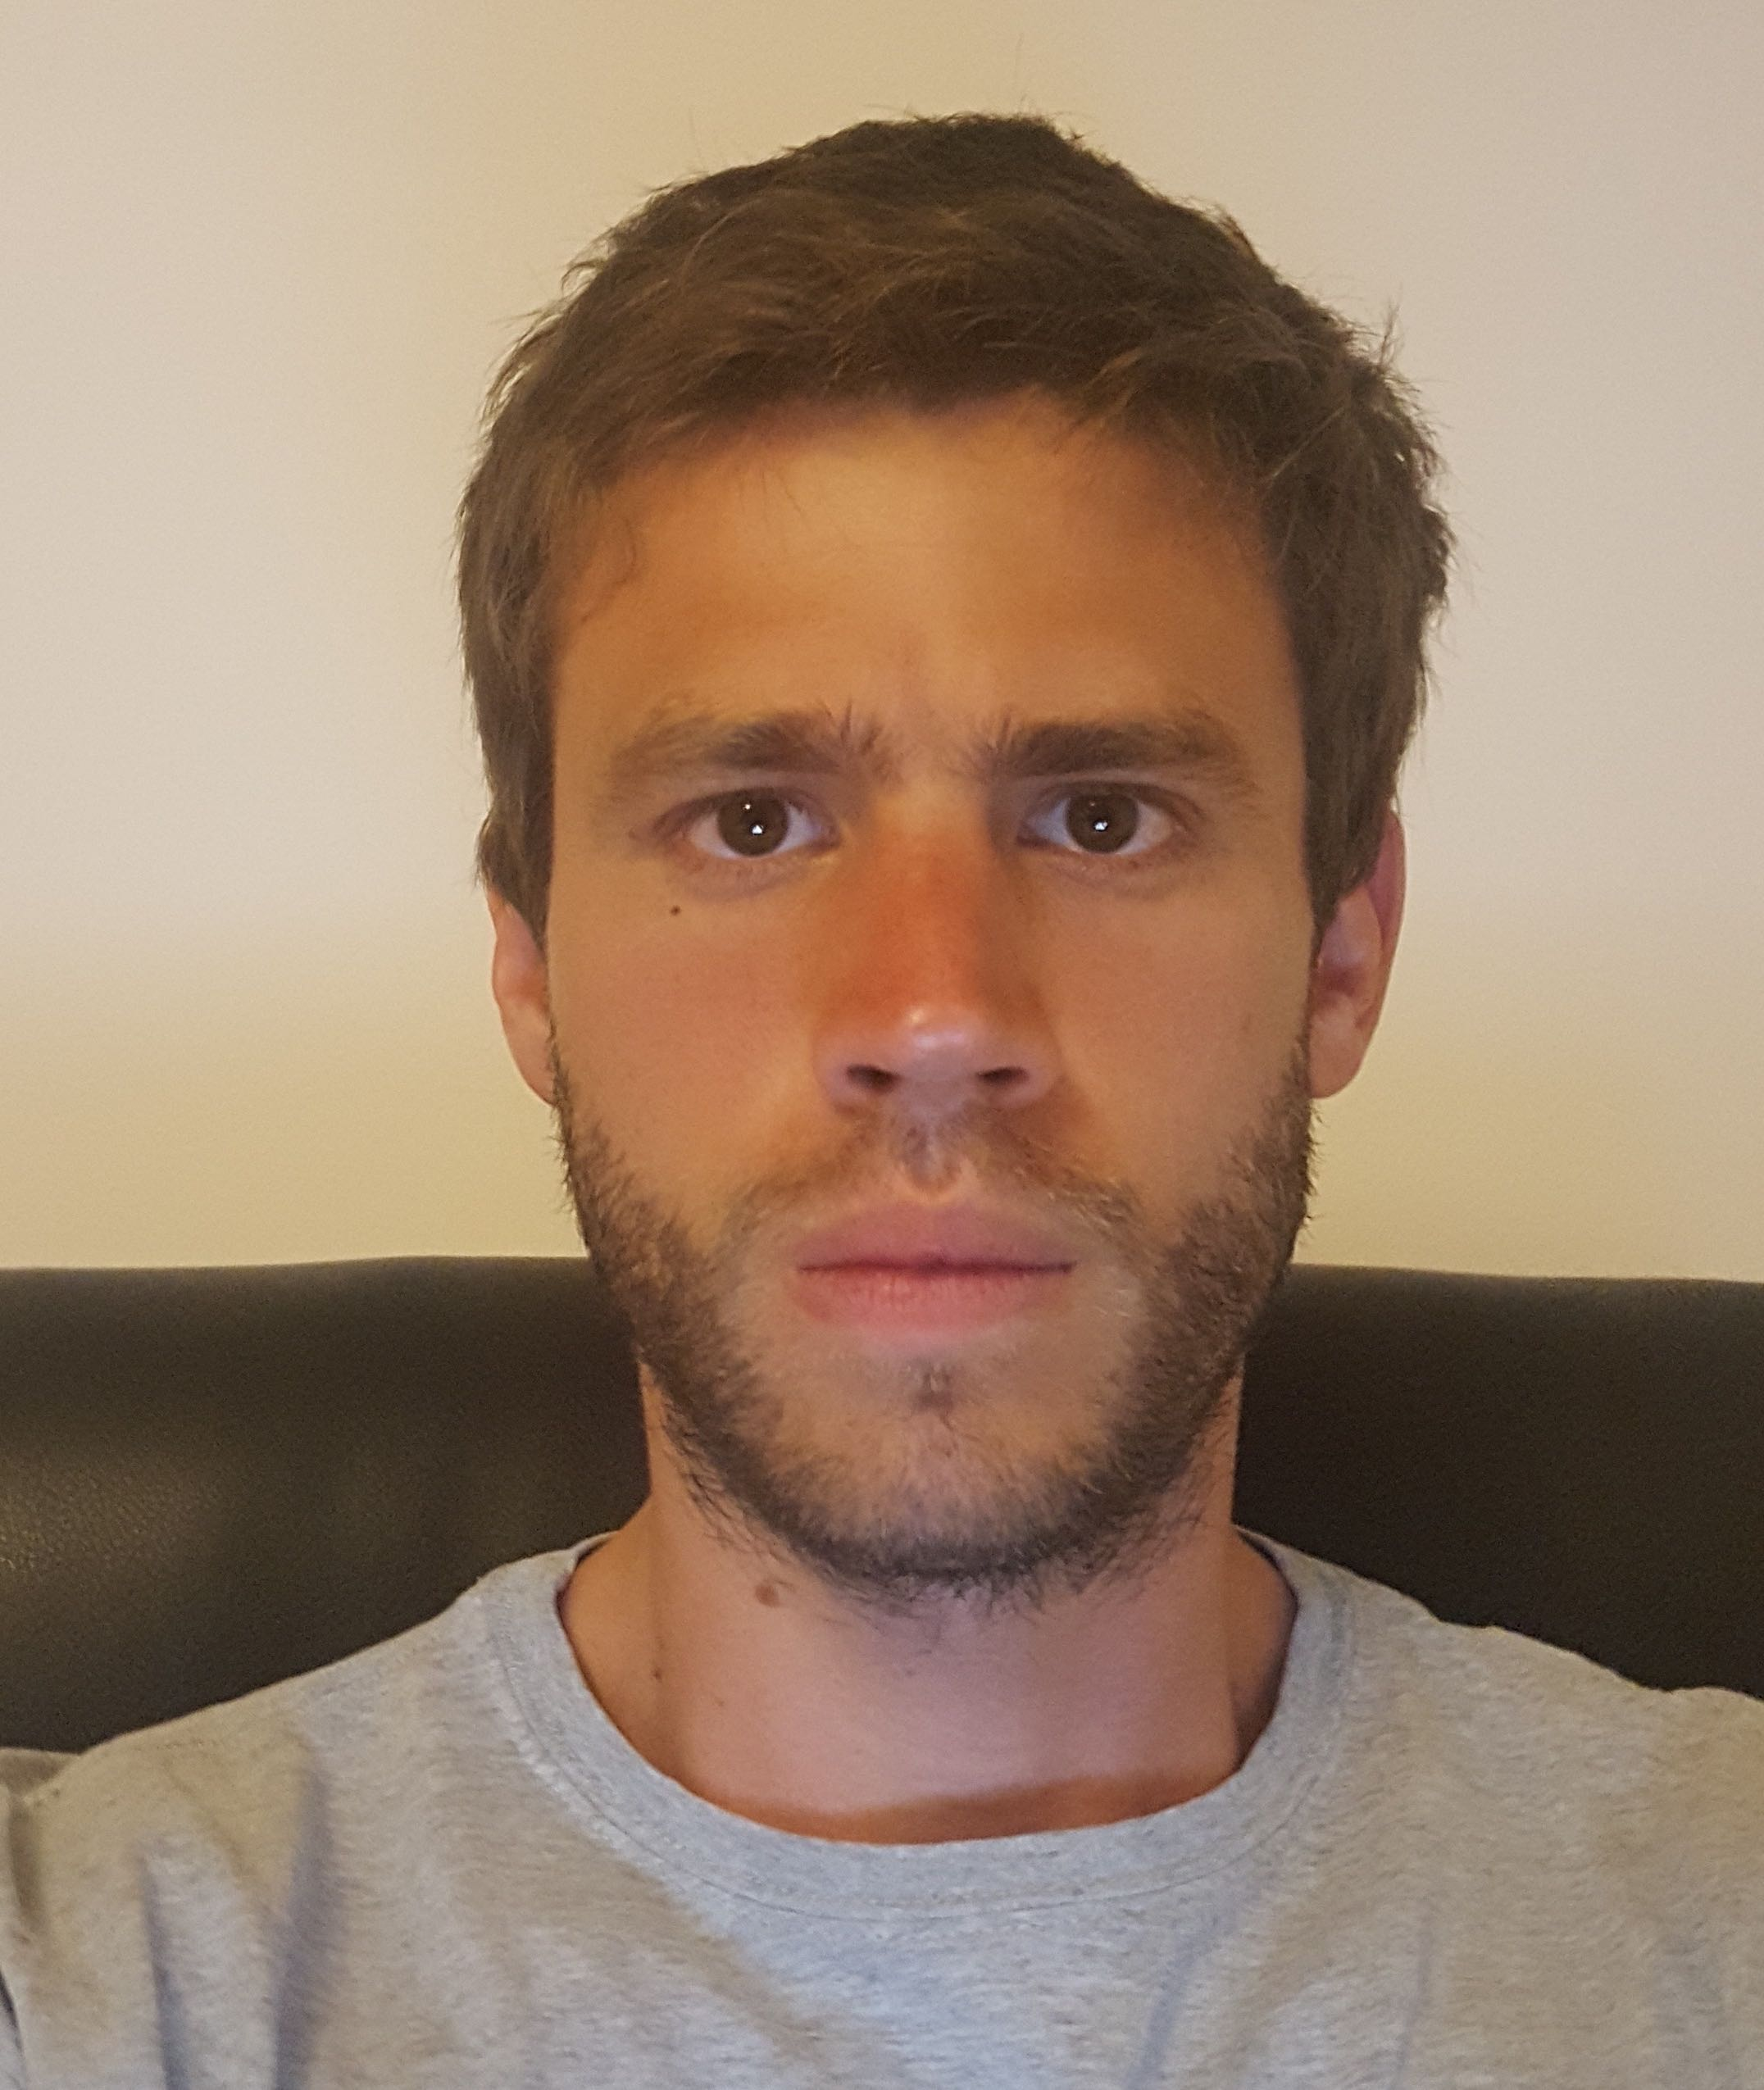
\includegraphics[width=3.5cm]{photos/photo-cv.jpg}\end{center}
\end{minipage}

% \vspace{1cm plus \grande minus \grande}

% -=-=-=-=-=-=-=-=-=-=-=-=-=-=-=-=-=-=-=-=-=-=-=-=-=-=-=-=-=-=-=-=-=-=-=-=-=-=-=-=-=-=
\begin{secciontrescol}{Academic Formation}

\filatresentres{2014}{%
\emph{MSc Nuclear Engineering}

Balseiro Institute, Cuyo National University \& National Atomic Energy Commission. San Carlos de Bariloche, Argentina.\\
GPA: 8.40/10.
}{\href{http://www.ib.edu.ar/english_version/Instituto_Balseiro.php}{
\includegraphics[width=0.8cm]{logos/ib}}}{-0.6cm}

\filasep

\filatresentres{2011}{%
Completed the first two years of Aeronautical Engineering.\\
National Technological University, Haedo Regional Faculty. Buenos Aires, Argentina.\\
GPA: 9.20/10.
}{\href{https://www.utn.edu.ar/es/}{
\includegraphics[width=0.8cm]{logos/utn}}}{-0.6cm}

\end{secciontrescol}

% \begin{secciondoscol}{Professional skills}
%  \filadosendos{}{Experience in mathematical modelling, numerical simulation and programming applied in both open source and proprietary software.}
% \end{secciondoscol}

% -=-=-=-=-=-=-=-=-=-=-=-=-=-=-=-=-=-=-=-=-=-=-=-=-=-=-=-=-=-=-=-=-=-=-=-=-=-=-=-=-=-=
\begin{secciontrescol}{Professional Experience}

\filatresentres{\scriptsize 2017 -- Current}{%
\azul{CRISIL}, Buenos Aires, Argentina \& New York, United States of America\\
\emph{Senior Quantitative Analyst}
}{\href{https://www.crisil.com}{
\includegraphics[width=0.9cm]{logos/crisil}}}{-0.6cm}

\filadosentres{}{
\begin{tabular}{rp{\anchoparrafo}}
 \textbf{Group}    & CRISIL Research \& Development \\
 \textbf{Location} & Buenos Aires, Argentina \\
 \textbf{Period}   & 2019 -- Current \\
\end{tabular}}%
\nopagebreak%

\filadosentres{}{%
\begin{itemize}
 \item Design, development, and coding of a derivative pricing engine using high-quality standards.
 \item Monte Carlo Methods for Stochastic Differential Equations following Peter E. Kloeden and Eckhard Platen book theory.
%  \item Interest Rate Modeling including Term Structure Models such as affine Short Rate models following Andersen .
 \item Interest Rate Modeling following both Leif B.G. Andersen, Vladimir V. Piterbarg and Damiano Brigo, Fabio Mercurio books theory.
\end{itemize}
}

\filadosentres{}{
\begin{tabular}{rp{\anchoparrafo}}
 \textbf{Client}   & Tier-1 US Bank -- Model Validation Group \\
 \textbf{Location} & New York, United States of America \\
 \textbf{Period}   & 2018 -- 2019 \\
\end{tabular}}%
\nopagebreak%

\filadosentres{}{%
\begin{itemize}
 \item Development of plausible future forecasts for macroeconomic and market variables in the context of Current Expected Credit Loss (CECL) models.
 \item Design, development, and maintenance of a forecasting suite implementing several methodologies in R.
\end{itemize}
}

\filadosentres{}{
\begin{tabular}{rp{\anchoparrafo}}
 \textbf{Client}   & Tier-1 US Bank -- Equity and Hybrids Group \\
 \textbf{Location} & Buenos Aires, Argentina \\
 \textbf{Period}   & 2017 -- 2018 \\
\end{tabular}}%
\nopagebreak%

\filadosentres{}{%
\begin{itemize}
 \item Price and risk management of Equity and Hybrid (IR/FX/COMM) exotic financial derivatives.
 \item Scrutiny of pricing methodology, model soundness and test suite design.
 \item Execution of calibration, benchmarking, computational performance, hedging, limiting cases, stability and convergence tests. CCAR stress testing and PAA explains.
 \item Responsible for technical documentation and executive summary report.
\end{itemize}
}

% \filasep

\filatresentres{2017 -- 2018}{%
\azul{BESNA}, Buenos Aires, Argentina\\
\emph{Engineering Consultant}
}{\href{http://www.besna.com.ar}{
\includegraphics[width=0.8cm]{logos/besna}}}{-0.6cm}

\filadosentres{}{
\begin{tabular}{rp{\anchoparrafo}}
 \textbf{Client}   & National Atomic Energy Commission (CNEA) \\
 \textbf{Project}  & Numerical Simulation of the CAREM-25 Steam Generator \\
 \textbf{Location} & Buenos Aires, Argentina \\
 \textbf{Period}   & 2017 -- 2018 \\
\end{tabular}}%
\nopagebreak%

\filadosentres{}{%
\begin{itemize}
 \item Design and development of Heat Transfer – Two-Phase Flow calculation codes for Nuclear Reactors.
\end{itemize}
}

% \filasep

\filatresentres{2014 -- 2017}{%
\azul{TECNA} Engineering Studies and Projects, Buenos Aires, Argentina \\
\emph{S/Sr Nuclear Engineer}
}{\href{http://www.tecna.com/Home/tabid/40/language/en-US/Default.aspx}{
\includegraphics[width=0.8cm]{logos/tecna-solo}}}{-0.6cm}

\filadosentres{}{
\begin{tabular}{rp{\anchoparrafo}}
 \textbf{Client}   & National Atomic Energy Commission (CNEA) \\
 \textbf{Project}  & CAREM-25 Balance of Plant \\
 \textbf{Location} & Buenos Aires, Argentina \\
 \textbf{Period}   & 2017 \\
\end{tabular}}%
\nopagebreak%

\filadosentres{}{%
\begin{itemize}
 \item Intermediary between the supplier and the client in topics related to nuclear aspects.
 \item Consultancy regarding operational modes of CAREM-25 reactor and their implications in the Balance of Plant (BOP).
\end{itemize}
}

\filadosentres{}{
\begin{tabular}{rp{\anchoparrafo}}
 \textbf{Client}   & Nucleoeléctrica Argentina S.A. \\
 \textbf{Project}  & Specialized Nuclear Engineering Services for CNAI-II \\
 \textbf{Location} & Buenos Aires, Argentina \\
 \textbf{Period}   & 2014 -- 2017 \\
\end{tabular}}%
\nopagebreak%

\filadosentres{}{%
\begin{itemize}
 \item Development of Reactor Physics (neutronic, thermohydraulic and control) calculation codes. 
 \item Detailed engineering projects for Nuclear Power Plants. 
 \item Specialist in calculations and analysis for Nuclear Reactors.
\end{itemize}
}

% \filasep

\filatresentres{2013 -- 2014}{%
\azul{INVAP S.E.}, Nuclear Engineering Department, San Carlos de Bariloche, Argentina \\
\emph{Undergraduate intern}
}{\href{http://www.invap.com.ar/en/}{
\includegraphics[width=0.8cm]{logos/invap}}}{-0.6cm}

\filadosentres{}{%
\begin{itemize}
 \item Nuclear engineering thesis: \href{http://ricabib.cab.cnea.gov.ar/467/}{\emph{Conceptual Design of a Compact Nuclear Research Reactor Core.}}
\end{itemize}
}

% \filasep
 
\filatresentres{2011 -- 2014}{%
\azul{CNEA} National Atomic Energy Commission, Bariloche Atomic Centre\\
\emph{Scholarship -- Student}
}{\href{http://www.cnea.gov.ar}{
\includegraphics[width=0.8cm]{logos/cnea}}}{-0.6cm}

\filadosentres{}{%
\begin{itemize}
 \item Studies carried out at the Balseiro Institute under the scholarship granted by the National Atomic Energy Commission to obtain the Nuclear Engineer title.
\end{itemize}
}

\end{secciontrescol}

% -=-=-=-=-=-=-=-=-=-=-=-=-=-=-=-=-=-=-=-=-=-=-=-=-=-=-=-=-=-=-=-=-=-=-=-=-=-=-=-=-=-=
\begin{secciondoscol}{Grants}

 \filadosendos{2011 -- 2014}{Scholarship from the National Atomic Energy Commission (CNEA) to study Nuclear Engineering at the Balseiro Institute.\\}

\end{secciondoscol}

% -=-=-=-=-=-=-=-=-=-=-=-=-=-=-=-=-=-=-=-=-=-=-=-=-=-=-=-=-=-=-=-=-=-=-=-=-=-=-=-=-=-=
\begin{secciondoscol}{Languages}
 \filadosendos{Spanish}{Native language.}
 \filadosendos{English}{Speaks, reads and writes fluently.}
\end{secciondoscol}

% -=-=-=-=-=-=-=-=-=-=-=-=-=-=-=-=-=-=-=-=-=-=-=-=-=-=-=-=-=-=-=-=-=-=-=-=-=-=-=-=-=-=
\begin{secciondoscol}{Programming and Software}
 \filadosendos{Languages}{C/C++/C\#, R, Python, FORTRAN, Scripting (bash, AWK, sed, curl, etc), \LaTeX, etc.}
 \filadosendos{Software}{GNU Scientific Library, PETSc, SLEPc, GNU Octave, Matlab, Mathematica, git, wasora, milonga, etc.}
\end{secciondoscol}

% -=-=-=-=-=-=-=-=-=-=-=-=-=-=-=-=-=-=-=-=-=-=-=-=-=-=-=-=-=-=-=-=-=-=-=-=-=-=-=-=-=-=
\begin{secciontrescol}{Open and Private software}

\software{wasora}{Wasora is a convenient high-level interface to perform mathematical computations. It also provides a framework which other particular computational codes can use. It is a free computational tool designed to aid a cognizant expert to analyze complex systems by solving mathematical problems by means of a high-level plain-text}{https://github.com/seamplex/wasora}

\software{milonga}{Milonga is a free core-level neutronic code that solves the steady-state multigroup neutron transport equation (using the diffusion approximation, discrete ordinates $S_N$ method or the method of characteristics) over unstructured grids (although simple structured grids can also be used) using either a finite-volumes or a finite-elements discretization scheme.}{https://bitbucket.org/rvignolo/milonga}

\software{mate}{Mate solves steady-state systems involving mixtures of steam and water (Two-Phase Flow) in different one dimensional, but still complex, geometries. Mass, Momentum, and Energy distributions are obtained through a finite difference scheme. It is intended to be free and open in the short term.}{https://github.com/rvignolo/mate}

\software{kosmos}{Kosmos is a derivative pricing engine in current and active development.}{https://github.com/rvignolo/kosmos}

\end{secciontrescol}

% -=-=-=-=-=-=-=-=-=-=-=-=-=-=-=-=-=-=-=-=-=-=-=-=-=-=-=-=-=-=-=-=-=-=-=-=-=-=-=-=-=-=
\vspace{\fill}
\hspace{0.6\linewidth}
\begin{minipage}{0.35\linewidth}
 \begin{center}
 Ramiro Vignolo\\
% version tracking
\immediate\write18{./date.sh > date.tex }
\immediate\write18{./hash.sh > hash.tex }

\makeatletter
\ifcase\pdf@shellescape
  \today\or
  \input{date}\or
  \today\fi

\scriptsize{\texttt{
\ifcase\pdf@shellescape
  unknown revision hash, re-compile with '--shell-escape'\or
  \input{hash}\or
  unknown revision hash, re-compile with '--shell-escape'\fi
}}
\makeatother
 
 \end{center}
\end{minipage}


\end{document}
